\documentclass[tikz,border=10pt]{standalone}
\usepackage{tkz-euclide} % 强化几何作图

\begin{document}
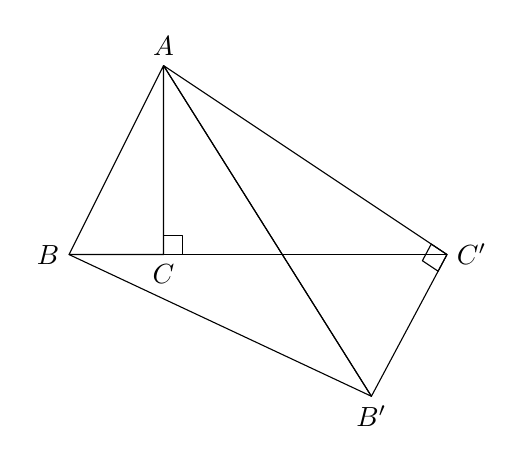
\begin{tikzpicture}[scale=1.2, line cap=round, line join=round]
    % 1. 定义核心点坐标 (基于图像比例估算)
    \coordinate (C) at (0,0);
    \coordinate (A) at (0,2);
    \coordinate (B) at (-1,0);
    
    % 2. 定义旋转后的点 (假设绕A旋转一定角度)
    % 也可以通过指定 C' 和 B' 的坐标来精确控制
    \coordinate (Cp) at (3,0); % C'
    \coordinate (Bp) at (2.2,-1.5); % B'
    
    % 3. 绘制实线部分 (三角形边和连接线)
    \draw(A) -- (B) -- (C) -- cycle; % 原始三角形 ABC
    \draw (C) -- (Cp);                % 连接 C 和 C'
    \draw (A) -- (Cp) -- (Bp) -- cycle; % 变换后的三角形 AB'C'
    \draw (B) -- (Bp);                % 连接 B 和 B'
    \draw (A) -- (Bp);                % 辅助线 AB'
    
    % 4. 绘制直角标记
    \tkzMarkRightAngle[size=0.2](A,C,Cp)      % 角 ACB 的直角标记
    \tkzMarkRightAngle[size=0.2](A,Cp,Bp)     % 角 AC'B' 的直角标记
    
    % 5. 标注字母标签
    \node[above] at (A) {$A$};
    \node[left] at (B) {$B$};
    \node[below] at (C) {$C$};
    \node[right] at (Cp) {$C'$};
    \node[below] at (Bp) {$B'$};
    
\end{tikzpicture}
\end{document}